\documentclass{beamer}
\beamertemplatenavigationsymbolsempty
\usetheme{default} \usecolortheme{default}
\usepackage[utf8]{inputenc}
\usepackage[T1]{fontenc}
%\usepackage{bera}
\usepackage[scaled]{beramono} %incosolata
\usepackage{tgheros}
\usepackage{longtable}
\usepackage{booktabs}
\usepackage{multicol} \setlength{\columnsep}{5mm}
\usepackage{xcolor}
\usepackage{listings}
\usepackage{hyperref}
\definecolor{mygreen}{rgb}{0,0.6,0}
\lstset{
    language=Java, 
    basicstyle=\ttfamily\scriptsize\selectfont,
    keywordstyle=\bfseries\color{blue},
    commentstyle=\color{mygreen},
    numberstyle={\footnotesize},
    numbers=none,
    backgroundcolor=\color{gray!10},
    frame=single,
    tabsize=4,
    rulecolor=\color{black!20},
    %title={\footnotesize\lstname},
  breaklines=false,
  breakatwhitespace=false,
    framextopmargin=2pt,
    framexbottommargin=2pt,
    showstringspaces=false,
}
\lstset{literate=%
%swedish and german letters
{Å}{{\AA}}1
{Ä}{{\"A}}1
{Ö}{{\"O}}1
{Ü}{{\"U}}1
{ß}{{\ss}}1
{ü}{{\"u}}1
{å}{{\aa}}1
{ä}{{\"a}}1
{ö}{{\"o}}1
%danish letters
{æ}{{\ae}}1
{ø}{{\o}}1
{Æ}{{\AE}}1
{Ø}{{\O}}1
}



\title{Föreläsning 1: Introduktion}
\author{Björn Regnell}
\institute{EDA016 Programmeringsteknik för D, LTH}
\date{HT Lp1-2, 2015}
 
\begin{document}
 
\frame{\titlepage}
\frame{\tableofcontents}

\frame{\frametitle{Kursens lärandemål}}
  
\frame{\frametitle{Vad är programmering?}}

\frame{\frametitle{Vad är Java?}}

\begin{frame}\frametitle{Hello World!}
\lstinputlisting[language=Java]{../../examples/src/lecture01intro/Hello.java}
\end{frame}

\frame{\frametitle{Undervisning}}

\frame{\frametitle{Kurslitteratur}
\begin{columns}
\begin{column}{0.6\textwidth}
\begin{itemize}
\item ''Objektorienterad programmering och Java" av Per Holm
\item Kurskompendium med övningar och laborationer
\item Bokpaket säljs på KFS John Ericssons väg 4 \url{http://www.kfsab.se/}
\end{itemize}
\end{column}
\begin{column}{0.5\textwidth}
\centering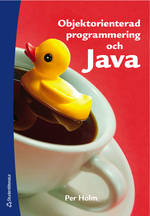
\includegraphics[width=0.5\textwidth]{../img/ankbok.jpg}
\end{column}
\end{columns}
}

\frame{\frametitle{Förkunskapsenkät}}

\frame{\frametitle{Samarbetsgrupper}}

 
\end{document}

